\section{Data dependent task-optimized streams}

In previous section we demonstrated that different tasks may need a different stream. For example, we saw
that PSNR stream significantly underperforms the histogram stream when applied to the histogram query.
Unfortunately, it is unclear what a best stream is for a given query. Moreover, it is common to stop analysis
task when the result is good enough, thus avoiding streaming all the data. Therefore, we define the best stream as
a sequence of refinements that reach the mininmum error at given stopping bit budget. Alas, in interactive application
we can only make assumptions what will be the number of bits streamed before user decides to stop the streaming. For
example, if a user drasticly changes viewpoint in a volume rendering application, the stream starts almost from scratch.

Taking the lack of control over the stopping budget to the extreme, the best stream becomes the one which minimizes
the error at all bit budgets. However, as in any global optimization problem we may get stuck at local minimum, as
chunks that improve the error but have impact on later refinement will have lower priority. The existence of local
minima prevents this progressive stream to be optimal.

Given above definition we can compute the optimal stream. It turns out that finding a permutation that minimizes
the total error given a bit budget is exponential in number of chunks. We thus use more practical greedy algorithm (is there
any approximation ratio?) that at each decision point one by one applies remaining chunks and computes the error
difference as if the chunk was not applied. We minimize the local minimum problem by taking the absolute value
of this difference which helps us to avoid a plateaus in the error curve.

\paragraph*{Coarse-to-fine greedy algorithm} starts with no data and the initial error is computed with respect
to the full data set. Then it takes a list of all chunks in the dataset, computes the error as if the chunk was
enabled, and picks the chunk with the highest absolute difference in the error with respect to the current error.
We use absolute difference to avoid the case where the error difference is zero or negative, which would result
in a long stream of chunk that do not decrease the error significantly. This assumption reflects the expectation
of more data meaning better result. The running time of this algorithm is $O(n^3)$ as we start with $n$ chunks
and at each streaming step decrease the chunk count by one. The cube factor comes from the need to perform inverse
wavelet transform and compute the error for each chunk.

\begin{figure}
        \centering
        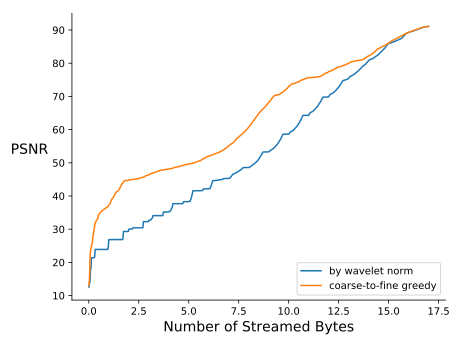
\includegraphics[width=0.48\linewidth]{img/figure4/rmse-miranda-viscosity}
        \includegraphics[width=0.48\linewidth]{img/figure4/histogram-miranda-viscosity}
        \caption{Comparison of coarse-to-fine and by wavelet norm streams on Miranda viscosity data set.
                 On the left is stream optimized for PSNR and on the right for histogram.}
\end{figure}

\paragraph*{Fine-to-coarse algorithm} is more practical as it utilizes full dataset to construct the stream.
This stream outperforms the coarse-to-fine greedy stream as it has access to more knowledge. Moreover,
if we wanted to precompute stream order which could be utilized during query, we would have access to whole
data set and could compute this stream. The algorithm is in principle a reverse of the previous approach, the
stream is constructed by starting with full data set and one by one disabling the chunks. At each step, a chunk
with smallest errorr impact is disabled (TODO: more detail). This algorithm is still of greedy nature as it
makes only locally optimal choice. Similarly to the coarse-to-fine algorithm, the running time is still $O(n^3)$.

\begin{figure}
        \centering
        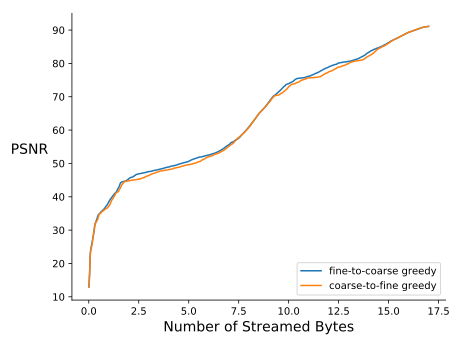
\includegraphics[width=0.48\linewidth]{img/figure5/rmse-miranda-viscosity}
        \includegraphics[width=0.48\linewidth]{img/figure5/histogram-miranda-viscosity}
        \caption{Comparison of coarse-to-fine and fine-to-coarse greedy algorithms on miranda viscosity data set.
                 On the left is stream optimized for PSNR and on the right for histogram.}
\end{figure}


As an optimization, we perform the error computation for each chunk only {\em once} and then sort these chunks
by the error. This approximation reduces the running time to $O(n^2)$ and thus makes it more practical (still
slow as hell) if
the stream order needs to be computed for a dataset, for example before the data is streamed over network.
Surprisingly, this stream is very close to the fully optimized stream which suggests the chunks do not drastically
affect each other.



\begin{figure}
        \centering
        \caption{The fine-to-coarse stream with only initial sorting closely follows the fully optimized stream.}
\end{figure}
